\chapter{Formal Analysis Using Alloy}
\label{chap:alloy_analysis}

\section{The Model Structure}
The formal Model has been developed using \textbf{Alloy 6}, leveraging its support for Linear Temporal Logic (LTL) to verify the dynamic behaviour of the System. The code is organized into modular files to enhance readability and maintainability: signatures, predicates, facts, assertions, and a main execution module.
The primary goal of this Model is to verify the correctness of the algorithm responsible for updating Segment status upon the publication of a Path, ensuring data consistency and isolation between Users.

\subsection{Signatures}
This module defines the structural atoms and the state of the System. A \emph{var} keyword is used to model mutable elements that evolve over time steps.
The representation abstracts away certain details to focus on the core verification goals:
\begin{itemize}
    \item \textbf{Users:} Only registered Users are modelled, as Guest Users operate in a read-only mode that does not alter the System state.
    \item \textbf{Obstacles:} These are omitted as they are static attributes in this context and do not influence the dynamic propagation of visibility and status logic.
    \item \textbf{PathEntries:} These are abstracted away. In the \hyperref[section:domain_class_diagram]{domain model}, a Path is composed of entries; in this formal Model, the Path's status is applied directly to the set of involved Segments. This abstraction simplifies the state space without compromising the logic of the propagation algorithm.
\end{itemize}

\begin{code}
    \inputminted{alloy}{code/signatures.als}
\end{code}

\subsection{Predicates}
This module outlines the possible state transitions (operations) within the System. A representative subset of actions has been selected to model the critical lifecycle of Paths and Trips.
Operations such as account deletion or unpublishing a Path are excluded from this abstraction. This design choice allows the Model to focus specifically on the \emph{safety} and \emph{liveness} properties of the publication workflow without the complexity of edge cases that do not affect the core update algorithm.
Each predicate defines strict pre-conditions and post-conditions to guide the solver.

\begin{code}
    \inputminted{alloy}{code/predicates.als}
\end{code}

\subsection{Facts}
This file contains the Model invariants and consistency conditions. These rules enforce:
\begin{itemize}
    \item \textbf{Structural Integrity:} Constraints that must hold true in every state (\eg, a Path must contain at least one Segment).
    \item \textbf{System Trace:} The definition of allowed temporal evolutions using LTL.
    \item \textbf{Consistency Conditions:} Rules ensuring that variables not explicitly modified by an operation remain unchanged (\emph{inertia}), preventing unwanted side effects.
\end{itemize}

\begin{code}
    \inputminted{alloy}{code/facts.als}
\end{code}

\subsection{Assertions}
This module encodes the properties that must be verified against the Model.
Rather than representing the full complexity of the real-world implementation, these assertions are tailored to the abstracted Model to formally prove:
\begin{itemize}
    \item \textbf{Safety:} Bad things never happen (\eg, a User cannot publish another User's Path).
    \item \textbf{Liveness:} Good things eventually happen (\eg, Segment status is updated correctly).
    \item \textbf{Possibility:} Valid states are reachable (\eg, Segment sharing between Paths is possible).
\end{itemize}

\begin{code}
    \inputminted{alloy}{code/assertions.als}
\end{code}

\subsection{Main Execution}
This file serves as the entry point for the Alloy Analyser. It contains the \texttt{run} commands to generate specific trace scenarios and the \texttt{check} commands to validate the assertions against the logic defined in the previous modules.

\begin{code}
    \inputminted{alloy}{code/main.als}
\end{code}

\newpage
\section{Validation through the Model}
This section illustrates the validation results obtained from the Alloy Analyzer. Instances generated by the \texttt{run} commands demonstrate the consistency of the Model, while the assertion checks verify the safety and liveness properties of the System.


\subsection{Large Static World}
The execution of the \texttt{run largeStaticWorld} command successfully produced a consistent instance, confirming that the structural axioms allow for a populated System state without contradictions.
Figure \ref{fig:large_static_model} depicts a meaningful snapshot of the System generated by the Analyser, featuring multiple Users, Paths, and Segments satisfying the multiplicity constraints.
\begin{figure}[H]
    \centering
    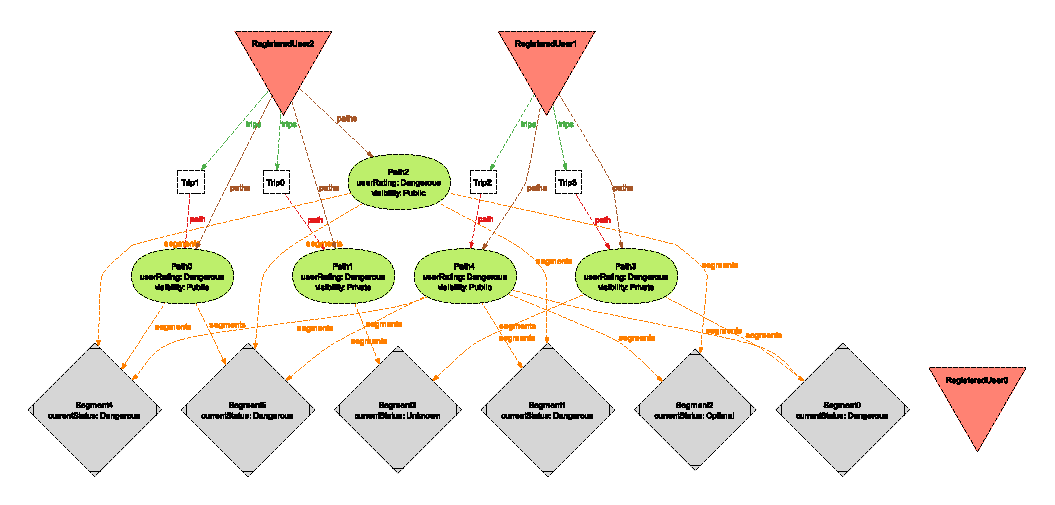
\includegraphics[width=\textwidth]{RASDv1.0/pdf/large_static_world.pdf}
    \caption{Large Static World Instance}
    \label{fig:large_static_model}
\end{figure}


\subsection{Dynamic World}
The \texttt{run dynamicWorld} command generates a trace satisfying the Linear Temporal Logic (LTL) specifications defined in the \emph{SystemTrace} fact. The following figures illustrate the step-by-step evolution of the System state.

\begin{figure}[H]
    \centering
    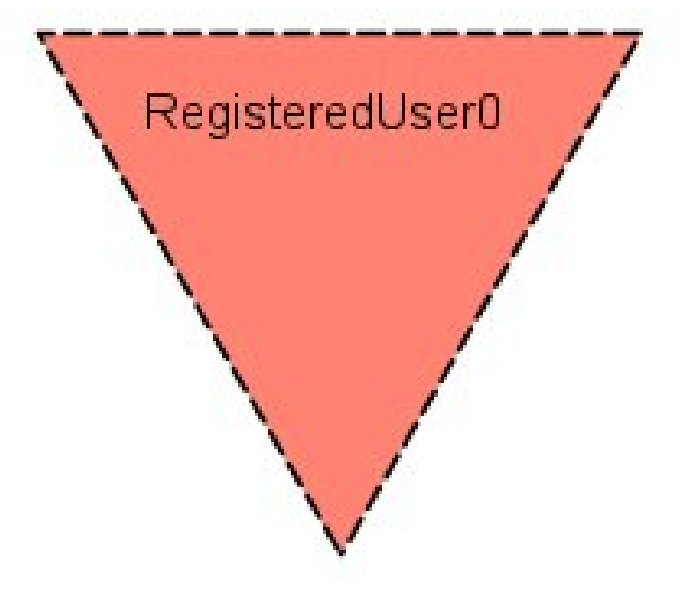
\includegraphics[width=0.2\textwidth]{RASDv1.0/pdf/dynamic_world_1.pdf}
    \caption{Dynamic World, Step 1: System Initialization and Sign Up}
    \label{fig:dynamic_1}
\end{figure}
\noindent
The trace begins in Figure \ref{fig:dynamic_1} with the initialization of the universe and the \texttt{signUp} of the first User.

\begin{figure}[H]
    \centering
    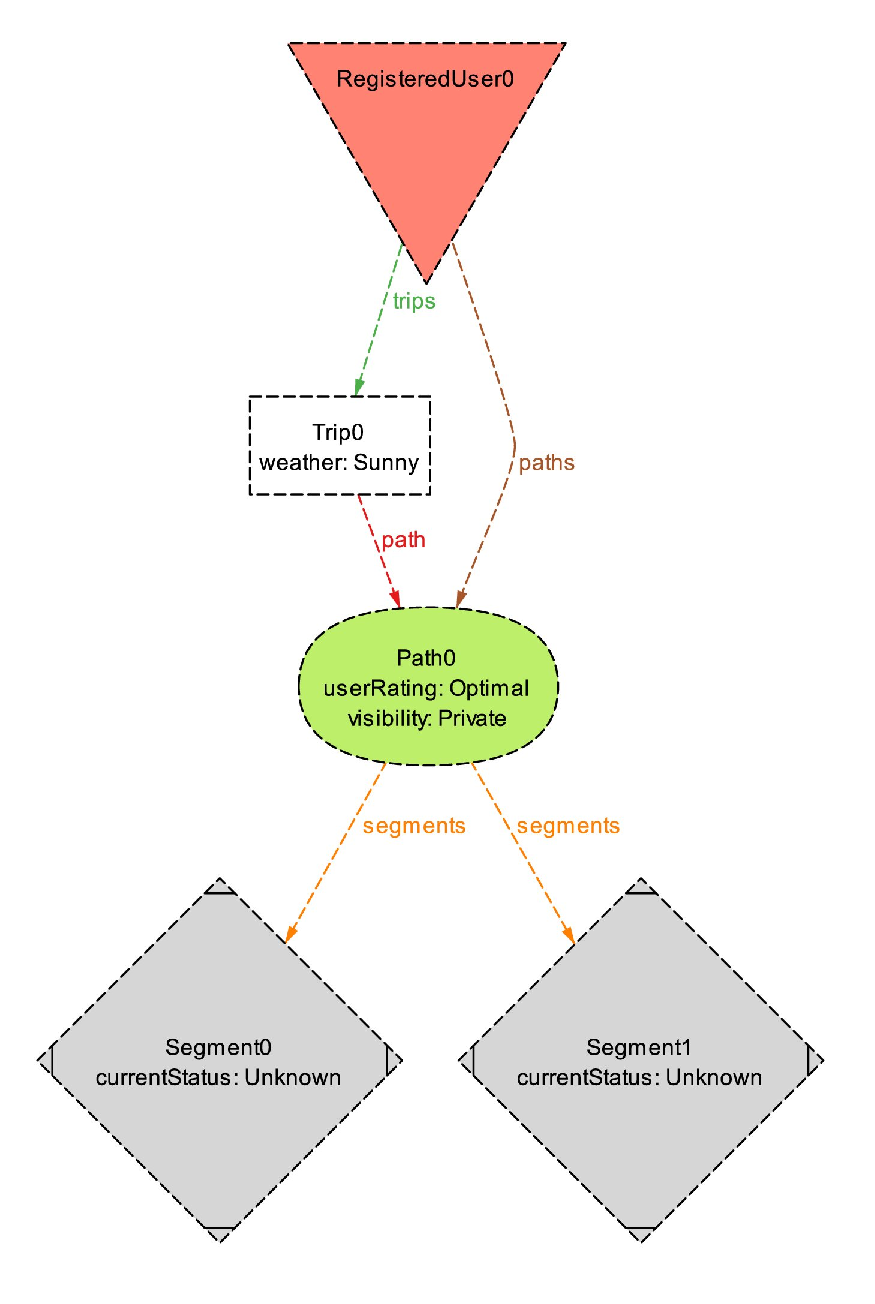
\includegraphics[width=0.4\textwidth]{RASDv1.0/pdf/dynamic_world_2.pdf}
    \caption{Dynamic World, Step 2: Trip Recording}
    \label{fig:dynamic_2}
\end{figure}
\noindent
In Figure \ref{fig:dynamic_2}, User 0 records a Trip. This action triggers the creation of a new Path and the instantiation of the corresponding Segments.

\begin{figure}[H]
    \centering
    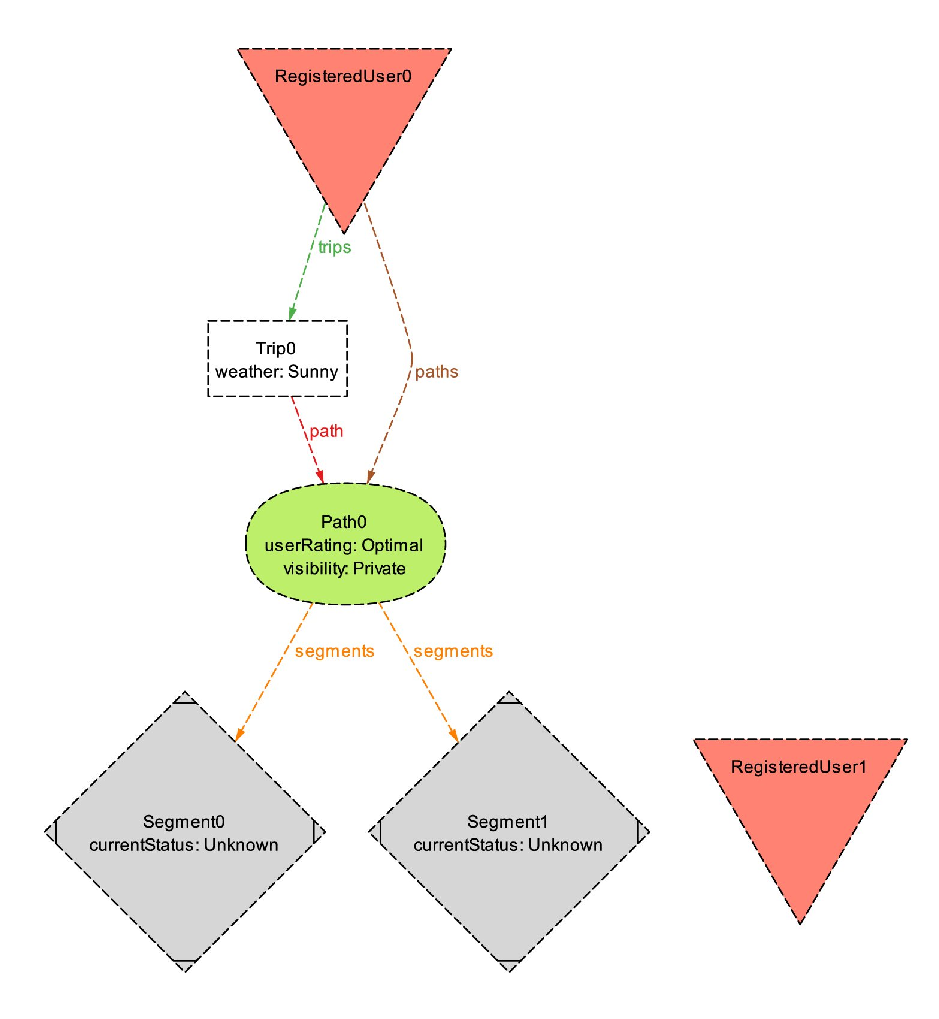
\includegraphics[width=0.5\textwidth]{RASDv1.0/pdf/dynamic_world_3.pdf}
    \caption{Dynamic World, Step 3: User 1 Sign Up}
    \label{fig:dynamic_3}
\end{figure}
\noindent
Figure \ref{fig:dynamic_3} shows the expansion of the User base with the registration of User 1.

\begin{figure}[H]
    \centering
    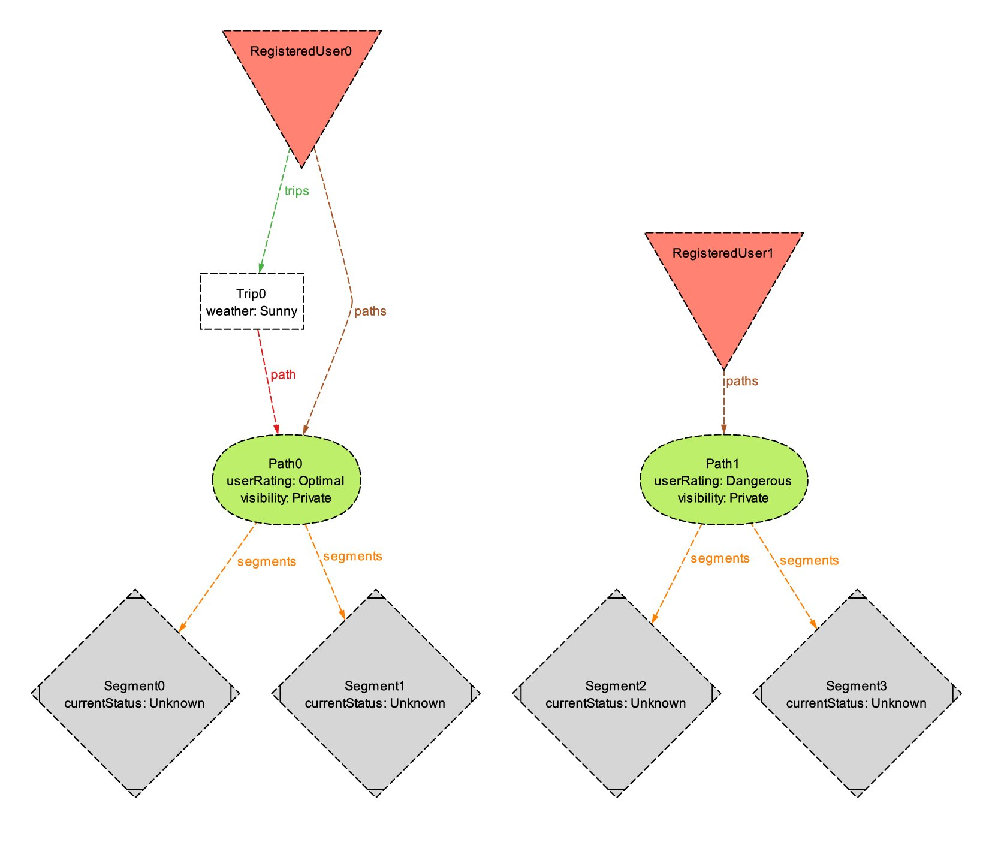
\includegraphics[width=0.7\textwidth]{RASDv1.0/pdf/dynamic_world_4.pdf}
    \caption{Dynamic World, Step 4: Manual Path Creation}
    \label{fig:dynamic_4}
\end{figure}
\noindent
In Figure \ref{fig:dynamic_4}, User 1 creates a manual Path. At this stage, the Path is private and its Segments are initialized with an \emph{Unknown} status.

\begin{figure}[H]
    \centering
    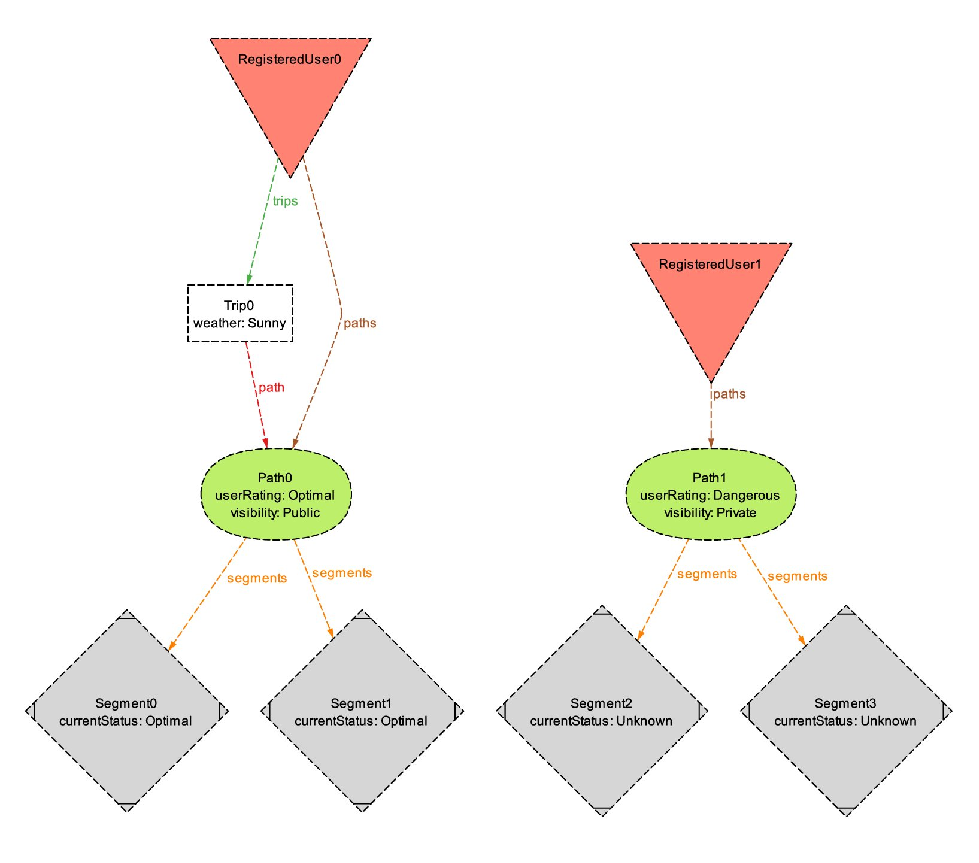
\includegraphics[width=0.7\textwidth]{RASDv1.0/pdf/dynamic_world_5.pdf}
    \caption{Dynamic World, Step 5: Path Publication}
    \label{fig:dynamic_5}
\end{figure}
\noindent
Figure \ref{fig:dynamic_5} illustrates the publication of User 0's Path. It is crucial to observe the side effect on the involved Segments: their status is updated from \emph{Unknown} to the rating provided by the User, propagating the information to the System.

\begin{figure}[H]
    \centering
    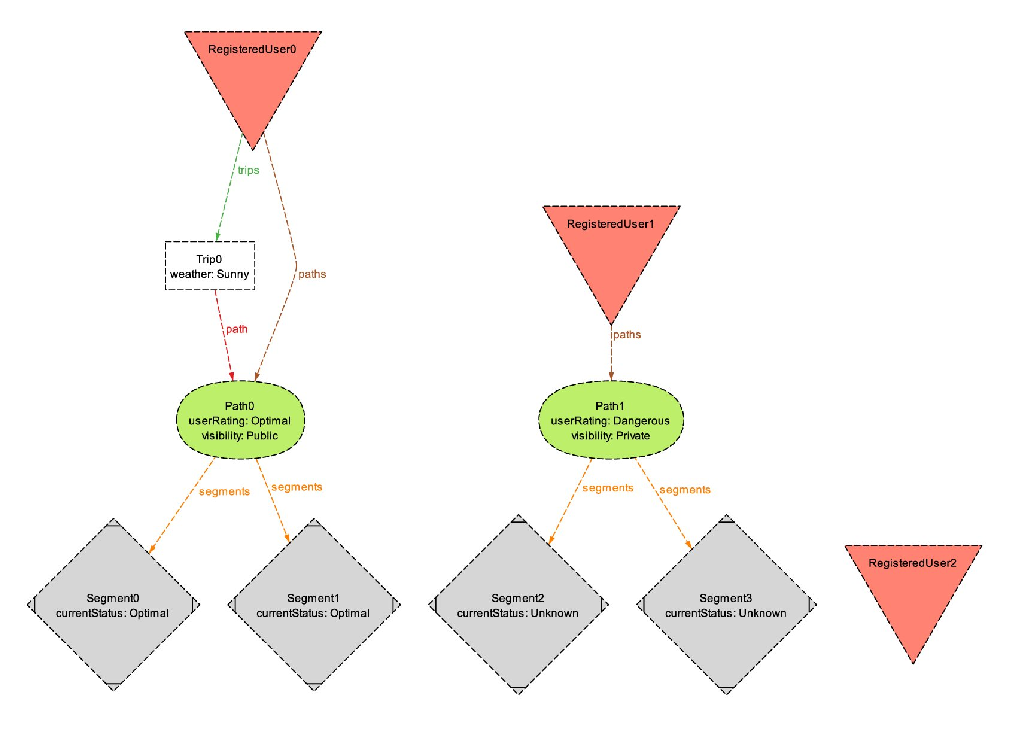
\includegraphics[width=0.85\textwidth]{RASDv1.0/pdf/dynamic_world_6.pdf}
    \caption{Dynamic World, Step 6: User 3 Sign Up}
    \label{fig:dynamic_6}
\end{figure}
\noindent
The scenario continues in Figure \ref{fig:dynamic_6} with the registration of a third User (User 3).

\begin{figure}[H]
    \centering
    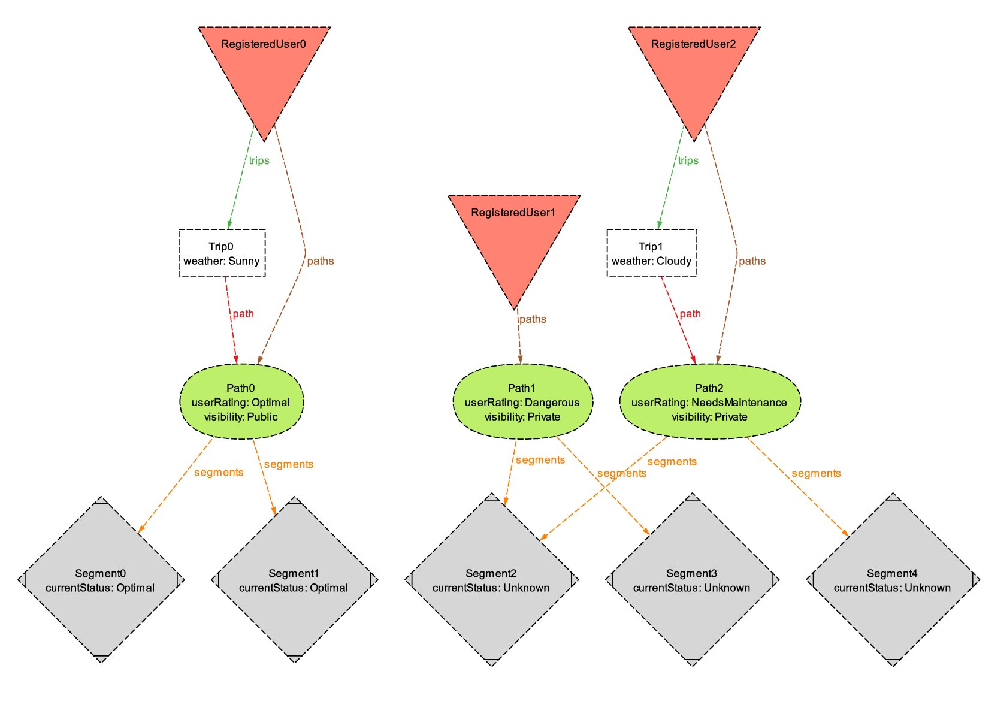
\includegraphics[width=0.85\textwidth]{RASDv1.0/pdf/dynamic_world_7.pdf}
    \caption{Dynamic World, Step 7: User 3 records a Trip}
    \label{fig:dynamic_7}
\end{figure}
\noindent
Figure \ref{fig:dynamic_7} highlights the Segment reuse logic. User 3 records a Trip that utilizes Segments already present in the System. Note that the private recording does not alter the status of these shared Segments, preserving the integrity of public data.

\begin{figure}[H]
    \centering
    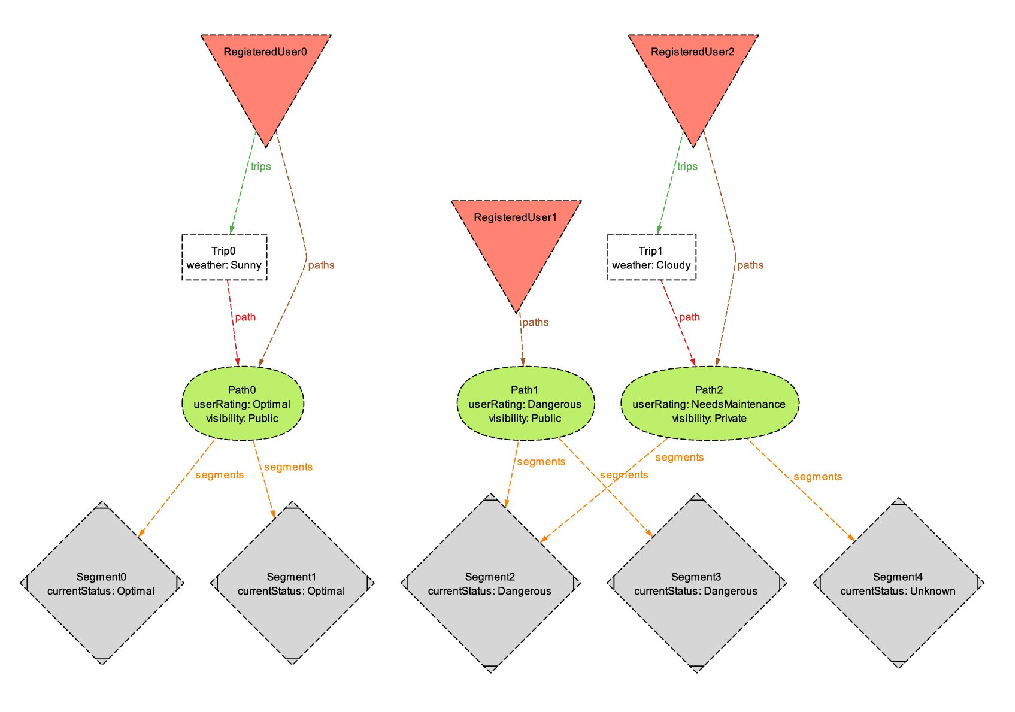
\includegraphics[width=0.9\textwidth]{RASDv1.0/pdf/dynamic_world_8.pdf}
    \caption{Dynamic World, Step 8: Second Publication}
    \label{fig:dynamic_8}
\end{figure}
\noindent
Figure \ref{fig:dynamic_8} shows the publication of User 1's Path, which updates the status of its specific Segments.

\begin{figure}[H]
    \centering
    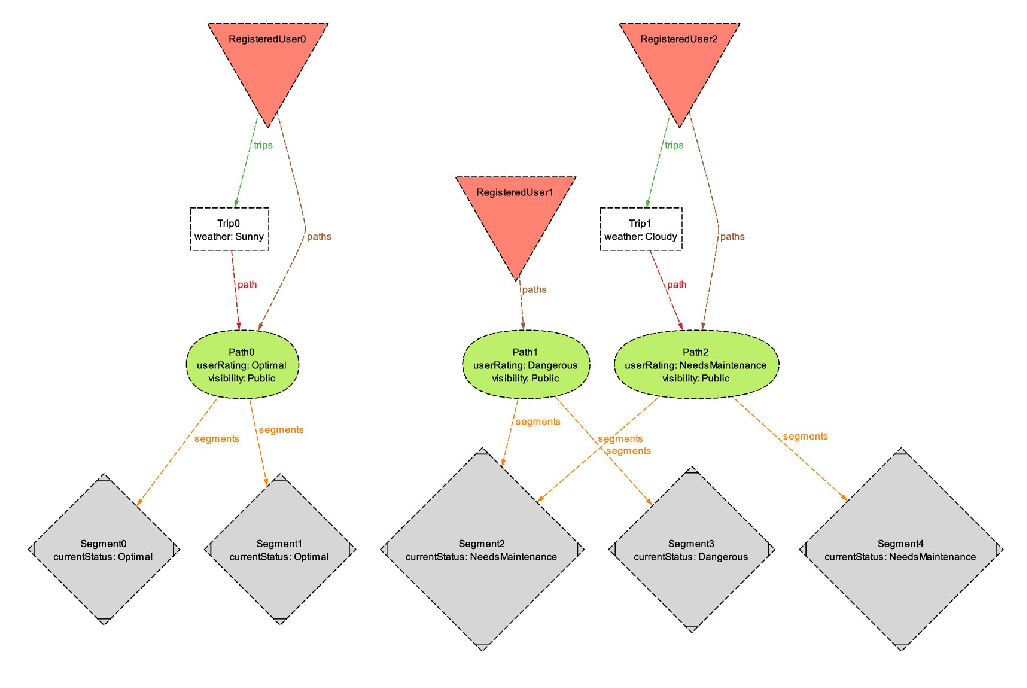
\includegraphics[width=0.9\textwidth]{RASDv1.0/pdf/dynamic_world_9.pdf}
    \caption{Dynamic World, Step 9: Third Publication}
    \label{fig:dynamic_9}
\end{figure}
\noindent
Finally, Figure \ref{fig:dynamic_9} shows the publication of User 2's Path, which updates the status of its specific Segments, overriding previous statuses, demonstrating that multiple publications can coexist without interference.

\subsection{Assertion Checks}
The formal properties of the Model were verified using the \texttt{check} command. The analyzer produced the following output:

\begin{code}
    \begin{minted}[frame=single]{alloy}
No counterexample found. VisibilityIsolation may be valid.
No counterexample found. SegmentsStatusSync may be valid.
No counterexample found. OncePublicAlwaysPublic may be valid.
Counterexample found. SharingIsImpossible is invalid.
    \end{minted}
\end{code}
\noindent
The results are fully consistent with the design requirements:
\begin{itemize}
    \item The absence of counterexamples for the first three assertions confirms the \textbf{Safety}, \textbf{Liveness}, and \textbf{Possibility} properties (isolation of User data, correct status synchronization, and monotonicity of public visibility).
    \item The counterexample found for \texttt{SharingIsImpossible} is a desired result and serves as a \textbf{constructive proof}. By refuting the impossibility of sharing, the Model demonstrates that states where Paths share Segments are reachable and valid, confirming the correct implementation of the reuse logic.
\end{itemize}